\def\thoigian{90}%--Thời gian
\de{ĐỀ THI GIỮA HỌC KỲ II NĂM HỌC 2023-2024}{THPT Thanh Bình 1 - Đồng Tháp}


\begin{center}
	\textbf{PHẦN 1 - TRẮC NGHIỆM}
\end{center}
\Opensolutionfile{ans}[ans/ans]

%Câu 1
\begin{ex}%[1D6N2-1]%[Dự án đề kiểm tra Toán 11 GHKI NH23-24 - Hiếu Mai]%[THPT Thanh Binh 1 - Tỉnh Đồng Tháp]
	Cho $a$ là số thực dương và $m$, $n$ là các số thực tùy ý. Mệnh đề nào sau đây \textbf{đúng}?
	\choice
	{$a^m \cdot a^n=\left(a^m \cdot a\right)^n$}
	{$a^m \cdot a^n=a^m+a^n$}
	{$a^m \cdot a^n=a^{m \cdot n}$}
	{\True $a^m \cdot a^n=a^{m+n}$}
	\loigiai{
		\lq\lq $a^m \cdot a^n=a^{m+n}$\rq\rq\, là mệnh đề đúng.
	}
\end{ex}

%Câu 2
\begin{ex}%[1D6N4-3]%[Dự án đề kiểm tra Toán 11 GHKI NH23-24 - Hiếu Mai]%[THPT Thanh Binh 1 - Tỉnh Đồng Tháp]
	Tập nghiệm của bất phương trình $\log x>1$ là
	\choice
	{$(-\infty ; 10)$}
	{\True $(10 ;+\infty)$}
	{$[10 ;+\infty)$}
	{$(0 ;+\infty)$}
	\loigiai{
		Ta có
		$$
		\log x>1
		\Leftrightarrow
		x>10^1
		\Leftrightarrow
		x>10.
		$$
		Vậy, bất phương trình đã cho có tập nghiệm là $(10 ;+\infty)$.
	}
\end{ex}

%Câu 3
\begin{ex}%[1H8H2-1]%[Dự án đề kiểm tra Toán 11 GHKI NH23-24 - Hiếu Mai]%[THPT Thanh Binh 1 - Tỉnh Đồng Tháp]
	Cho hình chóp đều $S . A B C D$ có đáy $A B C D$ là hình vuông tâm $O$. Khẳng định nào sau đây \textbf{đúng}?
	\choice
	{$S O \perp(S A B)$}
	{$S A \perp(S B D )$}
	{$S A \perp(A B C D)$}
	{\True $S O \perp(A B C D)$}
	\loigiai{
		\immini{
			Xét $ \triangle SAC $ cân tại $ S $ (do $ SA=SC $), ta thấy $ SO $ là trung tuyến và là đường cao. Do đó $ SO \perp AC $.
			\\
			Tương tự, ta cũng có $ SO \perp BD $.
			\\
			Vậy, $ SO \perp (ABCD) $.
		}
		{
			\begin{tikzpicture}[
				>=stealth, line join=round, line cap=round, 
				scale=.8,
				font=\footnotesize,
				declare function={r=3; a=75;}]
				% ve diem
				\path 
				(0,0) coordinate (A)
				($ (A)+(0:6) $) coordinate (B)
				($ (A)+(-135:3) $) coordinate (D)
				($ (B)+(D)-(A) $) coordinate (C)
				($ (B)!.5!(D) $) coordinate (O)
				($ (O)+(90:5) $) coordinate (S)
				;
				\draw[thick] 
				(C)--(S)--(D)--(C)--(B)--(S)
				;
				\draw[dotted] 
				(B)--(A)--(S)--(O)
				(C)--(A)--(D)--(B)
				;
				\foreach \x/\g in {A/150, B/30, C/-45, D/-135, S/90, O/-90}{
					\draw[fill=black] (\x) circle (1.5pt)+(\g:.4) node{$\x$};}
			\end{tikzpicture}
		}
	}
\end{ex}

%Câu 4
\begin{ex}%[1D6N2-2]%[Dự án đề kiểm tra Toán 11 GHKI NH23-24 - Hiếu Mai]%[THPT Thanh Binh 1 - Tỉnh Đồng Tháp]
	Cho hai số dương $a, b(a \neq 1)$. Mệnh đề nào dưới đây \textbf{sai}?
	\choice
	{$\log _a 1=0$}
	{$\log _a a^\alpha=\alpha$}
	{\True $\log _a a=2 a$}
	{$a^{\log _a b}=b$}
	\loigiai{
		Mệnh đề đúng phải là \lq\lq$\log _a a=1$\rq\rq.
	}
\end{ex}

%Câu 5
\begin{ex}%[1H8H1-3]%[Dự án đề kiểm tra Toán 11 GHKI NH23-24 - Hiếu Mai]%[THPT Thanh Binh 1 - Tỉnh Đồng Tháp]
	Cho hình chóp $S . A B C D$ có tất cả các cạnh bằng nhau. Góc giữa hai đường thẳng $S A$ và $B C$ bằng
	\choice
	{$90^{\circ}$}
	{\True $60^{\circ}$}
	{$45^{\circ}$}
	{$30^{\circ}$}
	\loigiai{
		\immini{
			Đáy $ ABCD $ có $ 4 $ cạnh bằng nhau nên nó là hình thoi. Suy ra $ BC \parallel AD $.
			\\
			Khi đó
			$$
			\left( BC;SA \right)
			=\left( AD;SA \right)
			=\widehat{SAD}
			=60^\circ.
			$$
			(do $ \triangle SAD $ đều).
		}
		{
			\begin{tikzpicture}[
				>=stealth, line join=round, line cap=round, 
				scale=.8,
				font=\footnotesize,
				declare function={r=3; a=75;}]
				% ve diem
				\path 
				(0,0) coordinate (A)
				($ (A)+(0:6) $) coordinate (B)
				($ (A)+(-135:3) $) coordinate (D)
				($ (B)+(D)-(A) $) coordinate (C)
				($ (B)!.5!(D) $) coordinate (O)
				($ (O)+(90:5) $) coordinate (S)
				;
				\draw[thick] 
				(C)--(S)--(D)--(C)--(B)--(S)
				;
				\draw[dotted] 
				(B)--(A)--(S)--(O)
				(C)--(A)--(D)--(B)
				;
				\foreach \x/\g in {A/150, B/30, C/-45, D/-135, S/90, O/-90}{
					\draw[fill=black] (\x) circle (1.5pt)+(\g:.4) node{$\x$};}
			\end{tikzpicture}
		}
	}
\end{ex}

%Câu 6
\begin{ex}%[1H8H1-3]%[Dự án đề kiểm tra Toán 11 GHKI NH23-24 - Hiếu Mai]%[THPT Thanh Binh 1 - Tỉnh Đồng Tháp]
	Cho hình lăng trụ $A B C \cdot A' B' C'$ có các đáy là các tam giác đều. Số đo của góc $\left(A B, B' C'\right)$ bằng
	\choice
	{$45^{\circ}$}
	{$90^{\circ}$}
	{\True $60^{\circ}$}
	{$30^{\circ}$}
	\loigiai{
		\immini{
			Do $ B'C' \parallel BC $ nên
			$$
			\left( AB;B'C' \right)
			=\left( AB;BC \right)
			=\widehat{ABC}
			=60^\circ.
			$$
			(do $ \triangle ABC $ đều).
		}
		{
			\begin{tikzpicture}[
				>=stealth, line join=round, line cap=round, 
				scale=.8,
				font=\footnotesize,
				declare function={r=3; a=75;}]
				% ve diem
				\path 
				(0,0) coordinate (A)
				($ (A)+(-45:3) $) coordinate (B)
				($ (A)+(0:6) $) coordinate (C)
				($ (A)+(80:5) $) coordinate (A')
				($ (A')+(B)-(A) $) coordinate (B')
				($ (A')+(C)-(A) $) coordinate (C')
				;
				\draw[thick] 
				(A')--(B')--(C')--cycle
				(A')--(A)
				(B')--(B)
				(C')--(C)
				(A)--(B)--(C)
				;
				\draw[dotted] 
				(A)--(C)
				;
				\foreach \a/\b/\c in {}	{
					\draw pic [draw=black,angle radius = 10] {right angle = \a--\b--\c};
				}
				%	\draw pic [draw, angle eccentricity=1.3, angle radius=20] {angle = S--C--A};
				\foreach \x/\g in {A/180, B/-75, C/0, A'/135, B'/-135, C'/45}{
					\draw[fill=black] (\x) circle (1.5pt)+(\g:.4) node{$\x$};}
			\end{tikzpicture}
		}
	}
\end{ex}

%Câu 7
\begin{ex}%[1H8H4-1]%[Dự án đề kiểm tra Toán 11 GHKI NH23-24 - Hiếu Mai]%[THPT Thanh Binh 1 - Tỉnh Đồng Tháp]
	Trong các khẳng định sau, khẳng định nào là khẳng định \textbf{sai}?
	\choice
	{\True Hai mặt phẳng phân biệt cùng vuông góc với một mặt phẳng thì song song với nhau}
	{Nếu một đường thẳng vuông góc với một trong hai đường thẳng song song thì cũng vuông góc với đường thẳng còn lại}
	{Hai mặt phẳng phân biệt cùng vuông góc với một đường thẳng thì song song với nhau}
	{Nếu một đường thẳng và một mặt phẳng (không chứa đường thẳng đó) cùng vuông góc với một đường thẳng thì song song với nhau}
	\loigiai{
		\lq\lq Hai mặt phẳng phân biệt cùng vuông góc với một mặt phẳng thì song song với nhau.\rq\rq\, là khẳng định sai.
	}
\end{ex}

%Câu 8
\begin{ex}%[1D6N3-3]%[Dự án đề kiểm tra Toán 11 GHKI NH23-24 - Hiếu Mai]%[THPT Thanh Binh 1 - Tỉnh Đồng Tháp]
	Hàm số nào dưới đây nghịch biến trên tập xác định của nó?
	\choice
	{$y=\left(\frac{\pi}{3}\right)^x$}
	{$y=\log _{\sqrt{3}} x$}
	{\True $y=\log _{\frac{\pi}{4}} x$}
	{$y=\log _2(\sqrt{x}+1)$}
	\loigiai{
		Hàm số $y=\log _{\frac{\pi}{4}} x$ là hàm log có cơ số $ \dfrac{\pi}{4} <1 $ nên nghịch biến trên tập xác định của nó.
	}
\end{ex}

%Câu 9
\begin{ex}%[1H8H4-1]%[Dự án đề kiểm tra Toán 11 GHKI NH23-24 - Hiếu Mai]%[THPT Thanh Binh 1 - Tỉnh Đồng Tháp]
	Cho hình chóp $S . A B C D$ có đáy $A B C D$ là hình vuông cạnh $a$, tâm $O, S A \perp(A B C D)$. Mệnh đề nào sau đây là đúng?
	\choice
	{$(S B C) \perp(S A D)$}
	{$(S B C) \perp(A B C D)$}
	{$(S B C) \perp(S C D)$}
	{\True $(S B C) \perp(S A B)$}
	\loigiai{
		\immini{
			Ta thấy
			$$
			\heva{&BC \perp AB \, \left( (ABCD) \text{ là hình vuông} \right) \\ &BC \perp SA \, \left( S A \perp(A B C D) \right)}
			\Rightarrow
			BC \perp (SAB).
			$$
			Mà $ BC \subset (SBC) $ nên $(S B C) \perp(S A B)$.
		}
		{
			\begin{tikzpicture}[
				>=stealth, line join=round, line cap=round, 
				scale=.8,
				font=\footnotesize,
				declare function={r=3; a=75;}]
				% ve diem
				\path 
				(0,0) coordinate (A)
				($ (A)+(0:6) $) coordinate (B)
				($ (A)+(-135:3) $) coordinate (D)
				($ (B)+(D)-(A) $) coordinate (C)
				($ (A)+(90:4) $) coordinate (S)
				;
				\draw[thick] 
				(C)--(S)--(D)--(C)--(B)--(S)
				;
				\draw[dotted] 
				(B)--(A)--(S)
				(A)--(D)
				;
				\foreach \a/\b/\c in {}	{
					\draw pic [draw=black,angle radius = 10] {right angle = \a--\b--\c};
				}
				%	\draw pic [draw, angle eccentricity=1.3, angle radius=20] {angle = S--C--A};
				\foreach \x/\g in {A/150, B/30, C/-45, D/-135, S/90}{
					\draw[fill=black] (\x) circle (1.5pt)+(\g:.4) node{$\x$};}
			\end{tikzpicture}
		}
	}
\end{ex}

%Câu 10
\begin{ex}%[1D6N1-1]%[Dự án đề kiểm tra Toán 11 GHKI NH23-24 - Hiếu Mai]%[THPT Thanh Binh 1 - Tỉnh Đồng Tháp]
	Với $a$ là số thực dương tùy ý, $\sqrt[2024]{a}$ bằng
	\choice
	{\True $a^{\frac{1}{2024}}$}
	{$a^{\sqrt{2024}}$}
	{$a^{2024}$}
	{$\sqrt{a^{2024}}$}
	\loigiai{
		Ta thấy $ \sqrt[2024]{a} = a^{\frac{1}{2024}} $.
	}
\end{ex}

%Câu 11
\begin{ex}%[1H8H1-3]%[Dự án đề kiểm tra Toán 11 GHKI NH23-24 - Hiếu Mai]%[THPT Thanh Binh 1 - Tỉnh Đồng Tháp]
	Cho hình lập phương $A B C D . A' B' C' D'$. Góc giữa $A' C'$ và $D B$ bằng
	\choice
	{\True $90^{\circ}$}
	{$30^{\circ}$}
	{$45^{\circ}$}
	{$60^{\circ}$}
	\loigiai{
		\immini{
			Do $A B C D . A' B' C' D'$ là hình lập phương nên $ ACC'A' $ là hình chữ nhật. Suy ra $ A'C' \parallel AC $.
			\\
			Khi đó
			$$
			\left( A'C';DB \right)
			=\left( AC;DB \right)
			=90^\circ.
			$$
		}
		{
			\begin{tikzpicture}[
				>=stealth, line join=round, line cap=round, 
				scale=.7,
				font=\footnotesize,
				declare function={r=3; a=75;}]
				% ve diem
				\path 
				(0,0) coordinate (A)
				($ (A)+(-135:3) $) coordinate (B)
				($ (A)+(0:6) $) coordinate (D)
				($ (B)+(D)-(A) $) coordinate (C)
				($ (A)+(90:5) $) coordinate (A')
				($ (A')+(B)-(A) $) coordinate (B')
				($ (A')+(C)-(A) $) coordinate (C')
				($ (A')+(D)-(A) $) coordinate (D')
				;
				\draw[thick] 
				(A')--(B')--(C')--(D')--cycle
				(B')--(B)
				(C')--(C)
				(D')--(D)
				(B)--(C)--(D)
				;
				\draw[dotted] 
				(A')--(A)
				(B)--(A)--(D)
				;
				\foreach \a/\b/\c in {}	{
					\draw pic [draw=black,angle radius = 10] {right angle = \a--\b--\c};
				}
				%	\draw pic [draw, angle eccentricity=1.3, angle radius=20] {angle = S--C--A};
				\foreach \x/\g in {A/135, B/-135, C/-45, D/0, A'/135, B'/-150, C'/-45, D'/45}{
					\draw[fill=black] (\x) circle (1.5pt)+(\g:.4) node{$\x$};}
			\end{tikzpicture}
		}
	}
\end{ex}

%Câu 12
\begin{ex}%[1D6N3-3]%[Dự án đề kiểm tra Toán 11 GHKI NH23-24 - Hiếu Mai]%[THPT Thanh Binh 1 - Tỉnh Đồng Tháp]
	Tìm hàm số đồng biến trên $\mathbb{R}$.
	\choice
	{$f(x)=3^{-x}$}
	{$f(x)=\dfrac{3}{3^x}$}
	{\True $f(x)=3^x$}
	{$f(x)=\left(\dfrac{1}{\sqrt{3}}\right)^x$}
	\loigiai{
		Hàm số $f(x)=3^x$ là hàm mũ dạng $ y=a^x $ với $ a=3>1 $ nên đồng biến trên $\mathbb{R}$.
	}
\end{ex}

%Câu 13
\begin{ex}%[1H8H2-2]%[Dự án đề kiểm tra Toán 11 GHKI NH23-24 - Hiếu Mai]%[THPT Thanh Binh 1 - Tỉnh Đồng Tháp]
	Cho hình chóp $S . A B C D$ có $S A \perp(A B C D)$ và đáy là hình vuông. Khẳng định nào sau đây là đúng?
	\choice
	{$A C \perp(S A B)$}
	{\True $B C \perp(S A B)$}
	{$A C \perp(S B D)$}
	{$A C \perp(S A D)$}
	\loigiai{
		\immini{
			Ta thấy
			$$
			\heva{&BC \perp AB \, \left( (ABCD) \text{ là hình vuông} \right) \\ &BC \perp SA \, \left( S A \perp(A B C D) \right)}
			\Rightarrow
			BC \perp (SAB).
			$$
		}
		{
			\begin{tikzpicture}[
				>=stealth, line join=round, line cap=round, 
				scale=.8,
				font=\footnotesize,
				declare function={r=3; a=75;}]
				% ve diem
				\path 
				(0,0) coordinate (A)
				($ (A)+(0:6) $) coordinate (B)
				($ (A)+(-135:3) $) coordinate (D)
				($ (B)+(D)-(A) $) coordinate (C)
				($ (A)+(90:4) $) coordinate (S)
				;
				\draw[thick] 
				(C)--(S)--(D)--(C)--(B)--(S)
				;
				\draw[dotted] 
				(B)--(A)--(S)
				(C)--(A)--(D)--(B)
				;
				\foreach \a/\b/\c in {}	{
					\draw pic [draw=black,angle radius = 10] {right angle = \a--\b--\c};
				}
				%	\draw pic [draw, angle eccentricity=1.3, angle radius=20] {angle = S--C--A};
				\foreach \x/\g in {A/150, B/30, C/-45, D/-135, S/90}{
					\draw[fill=black] (\x) circle (1.5pt)+(\g:.4) node{$\x$};}
			\end{tikzpicture}
		}
	}
\end{ex}

%Câu 14
\begin{ex}%[1H8H2-1]%[Dự án đề kiểm tra Toán 11 GHKI NH23-24 - Hiếu Mai]%[THPT Thanh Binh 1 - Tỉnh Đồng Tháp]
	Trong các khẳng định sau, khẳng định nào là khẳng định \textbf{đúng}?
	\choice
	{$a \perp(P) \Rightarrow a \perp b$}
	{$\heva{&a \perp b \\ &a \perp c} \Rightarrow a \perp(P)$}
	{$\heva{&a \perp b \\ &b \perp c} \Rightarrow a \parallel c$}
	{\True $\heva{&a \perp b \\ &a \perp c \\ &b \cap c=\{O\} \\ &b, c \subset(P)} \Rightarrow a \perp(P)$}
	\loigiai{
		Dễ thấy
		$$
		\heva{&a \perp b \\ &a \perp c \\ &b \cap c=\{O\} \\ &b, c \subset(P)} \Rightarrow a \perp(P)
		$$ là khẳng định đúng.
	}
\end{ex}

%Câu 15
\begin{ex}%[1D6H2-1]%[Dự án đề kiểm tra Toán 11 GHKI NH23-24 - Hiếu Mai]%[THPT Thanh Binh 1 - Tỉnh Đồng Tháp]
	Cho $a>0$, $a \neq 1$, biểu thức $D=\log _{a^3} a$ có giá trị bằng bao nhiêu?
	\choice
	{\True $\dfrac{1}{3}$}
	{$ -3 $}
	{$-\dfrac{1}{3}$}
	{$ 3 $}
	\loigiai{
		Ta có
		$$
		D=\log _{a^3} a
		=\dfrac{1}{3} \log_a a
		=\dfrac{1}{3}.
		$$
	}
\end{ex}

%Câu 16
\begin{ex}%[1D6N4-2]%[Dự án đề kiểm tra Toán 11 GHKI NH23-24 - Hiếu Mai]%[THPT Thanh Binh 1 - Tỉnh Đồng Tháp]
	Phương trình $2^{x-1}=4$ có nghiệm là
	\choice
	{$x=17$}
	{\True $x=3$}
	{$x=1$}
	{$x=2$}
	\loigiai{
		Ta có
		$$
		2^{x-1}=4
		\Leftrightarrow
		x-1=2
		\Leftrightarrow
		x=3.
		$$
		Vậy phương trình đã cho có nghiệm $ x=3 $.
	}
\end{ex}


\Closesolutionfile{ans}
%\begin{center}
%	\textbf{ĐÁP ÁN}
%	\inputansbox{10}{ans/ans}	
%\end{center}



\begin{center}
	\textbf{PHẦN 2 - ĐÚNG SAI}
\end{center}

\Opensolutionfile{ans}[ans/answer]
% cau 1
\begin{ex}%[1D6H1-1]%[Dự án đề kiểm tra Toán 11 GHKI NH23-24 - Hiếu Mai]%[THPT Thanh Binh 1 - Tỉnh Đồng Tháp]
	Hãy nhận xét tính \textbf{Đúng} - \textbf{Sai} của mỗi nhận định sau.
	\choiceTF[1t]
	{\True $Q=a^{\frac{2}{3}} \sqrt{a}=a^{\frac{7}{6}}, a>0$}
	{$P=6^{\sqrt{7}} \cdot 6^{2-\sqrt{7}}=6$}
	{\True Cho $x>0, y>0$. Viết biểu thức $x^{\frac{4}{5}} \cdot \sqrt[6]{x^5 \sqrt{x}}$ về dạng $x^m$ và biểu thức $y^{\frac{4}{5}}: \sqrt[6]{y^5 \sqrt{y}}$ về dạng $y^n$.
		\\
		Ta được: $m-n=\frac{11}{6}$}
	{\True Với $a, b>0, \ln (a b)=\ln a+\ln b$}
	\loigiai{
		\begin{itemchoice}
			\itemch $Q=a^{\frac{2}{3}} \sqrt{a}= a^{\frac{2}{3}} \cdot a^{\frac{1}{2}} = a^{\frac{2}{3}+\frac{1}{2}} = a^{\frac{7}{6}} $.
			\itemch $P=6^{\sqrt{7}} \cdot 6^{2-\sqrt{7}}=6^2=36$.
			\itemch Ta có
			\begin{align*}
				&x^{\frac{4}{5}} \cdot \sqrt[6]{x^5 \sqrt{x}}
				= x^{\frac{4}{5}} \cdot \sqrt[6]{x^5 x^{\frac{1}{2}}}
				= x^{\frac{4}{5}} \cdot \sqrt[6]{x^{\frac{11}{2}}}
				= x^{\frac{4}{5}} \cdot x^{\frac{11}{12}}
				= x^{\frac{4}{5}+\frac{11}{12}} \\
				&y^{\frac{4}{5}} \colon \sqrt[6]{y^5 \sqrt{y}}
				= y^{\frac{4}{5}} \colon \sqrt[6]{y^5 y^{\frac{1}{2}}}
				= y^{\frac{4}{5}} \colon \sqrt[6]{y^{\frac{11}{2}}}
				= y^{\frac{4}{5}} \colon y^{\frac{11}{12}}
				= y^{\frac{4}{5}-\frac{11}{12}}
			\end{align*}
			Do đó
			$$
			m-n = \dfrac{4}{5}+\dfrac{11}{12} - \left( \dfrac{4}{5}-\dfrac{11}{12} \right)
			= \dfrac{11}{6}.
			$$
			\itemch Với $a, b>0, \ln (a b)=\ln a+\ln b$.
		\end{itemchoice}
	}
\end{ex}

% cau 2
\begin{ex}%[1H8H2-2]%[Dự án đề kiểm tra Toán 11 GHKI NH23-24 - Hiếu Mai]%[THPT Thanh Binh 1 - Tỉnh Đồng Tháp]
	Cho tứ diện đều $A B C D$. Gọi $H$ là trọng tâm tam giác $A B C$. Khi đó
	\choiceTF[1t]
	{\True $A D$ và $B C$ vuông góc với nhau}
	{\True $D H$ vuông góc với $(A B C)$}
	{\True $H$ là hình chiếu vuông góc của $D$ lên $(A B C)$}
	{$D A$ vuông góc với $(A B C)$}
	\loigiai{
		\begin{center}
			\begin{tikzpicture}[
				>=stealth, line join=round, line cap=round, 
				scale=1,
				declare function={r=3; a=75;}]
				% ve diem
				\path 
				(0,0) coordinate (B)
				($ (B)+(-55:3) $) coordinate (C)
				($ (B)+(0:6) $) coordinate (D)
				($ (C)!.5!(D) $) coordinate (N)
				($ (B)!2/3!(N) $) coordinate (O)
				($ (O)+(90:4) $) coordinate (A)
				($ (C)!.5!(B) $) coordinate (M)
				($ (A)!{2/3}!(M) $) coordinate (H)
				;
				\draw[thick] 
				(A)--(B)--(C)--(A)--(D)--(C)
				(A)--(M)
				;
				\draw[dotted] 
				(B)--(D)--(M)
				(B)--(N)
				(A)--(O)
				(D)--(H)
				;
				\foreach \a/\b/\c in {}	{
					\draw pic [draw=black,angle radius = 10] {right angle = \a--\b--\c};
				}
				%	\draw pic [draw, angle eccentricity=1.3, angle radius=20] {angle = S--C--A};
				\foreach \x/\g in {A/90, B/180, C/-60, D/0, H/135, O/-90, M/-135}{
					\draw[fill=black] (\x) circle (1.5pt)+(\g:.4) node{$\x$};}
			\end{tikzpicture}
		\end{center}
		\begin{itemchoice}
			\itemch
			Gọi $ O $ là trọng tâm $ \triangle BCD $; $ M $ là trung điểm $ BC $.
			Dễ thấy $ BC \perp AM $ ($ \triangle ABC $ đều) và $ BC \perp DM $ ($ \triangle BCD $ đều) nên $ BC \perp (ADM) $.
			\\
			Mà $ AD \subset (ADM) $ nên $ BC \perp AD $.
			\itemch
			Do $ ABCD $ là tứ diện đều có $ H $ là trọng tâm $ \triangle ABC $ nên $ DH $ là một đường cao của tứ diện này.
			\\
			Do đó $ DH \perp (ABC) $.
			\itemch
			Do $ DH \perp (ABC) $ và $ H \in (ABC) $ nên $ H $ là hình chiếu của $ D $ lên $ (ABC) $.
			\itemch
			Do $ H $ là hình chiếu của $ D $ lên $ (ABC) $ nên góc tạo bởi đường $ DA $ và mặt phẳng $ (ABC) $ là
			$$
			\left( DA;AH \right)
			\ne 90^\circ
			$$
			Vậy $ DA \not\perp (ABC) $.
		\end{itemchoice}
	}
\end{ex}

% cau 3
\begin{ex}%[1D6H3-3]%[Dự án đề kiểm tra Toán 11 GHKI NH23-24 - Hiếu Mai]%[THPT Thanh Binh 1 - Tỉnh Đồng Tháp]
	Cho hàm số $y=\log _{\sqrt{2}}\left(x^2-2 x-3\right)$ có tập xác định là $\mathscr{D}$.
	\choiceTF[1t]
	{Đồ thị hàm số đi qua điểm $M(-2 ; 2)$}
	{$\log _{\sqrt{2}}\left(x^2-2 x-3\right)=\log _2 \sqrt{x^2-2 x-3}, \forall x \in D$}
	{\True Tập xác định của hàm số là $\mathscr{D}=(-\infty ;-1) \cup(3 ;+\infty)$}
	{\True Đồ thị hàm số cắt trục hoành tại điểm có hoành độ $x=1 \pm \sqrt{5}$}
	\loigiai{
		\begin{itemchoice}
			\itemch 
			Thay tọa độ điểm $M(-2 ; 2)$ vào hàm số $y=\log _{\sqrt{2}}\left(x^2-2 x-3\right)$, ta được
			$$
			2=\log _{\sqrt{2}}\left(4+4-3\right) \quad \text{(sai)}.
			$$
			Vậy, điểm $ M $ không thuộc đồ thị của hàm số.
			\itemch Ta thấy
			$$ 
			\log _{\sqrt{2}}\left(x^2-2 x-3\right)=\log _2 \left( x^2-2 x-3 \right)^2, \forall x \in \mathscr{D}.
			$$
			\itemch
			Hàm số xác định khi
			$$
			x^2-2 x-3 >0
			\Leftrightarrow
			\hoac{&x<-1 \\&x>3.}
			$$
			Do đó tập xác định của hàm số là $\mathscr{D}=(-\infty ;-1) \cup(3 ;+\infty)$.
			\itemch
			Cho $ y=0 $, ta được
			$$	
			\log _{\sqrt{2}}\left(x^2-2 x-3\right) = 0
			\Leftrightarrow
			x^2-2 x-3 =1
			\Leftrightarrow
			x=1 \pm \sqrt{5}.
			$$
			Vậy, đồ thị hàm số cắt trục hoành tại điểm có hoành độ $x=1 \pm \sqrt{5}$.
		\end{itemchoice}
	}
\end{ex}


\Closesolutionfile{ans}
%\inputansbox[2]{2}{ans/answer.tex}

\begin{center}
	\textbf{PHẦN 3 - TỰ LUẬN}
\end{center}

%Câu 1...........................
\begin{bt}%[1D6H4-2]%[Dự án đề kiểm tra Toán 11 GHKI NH23-24- Nguyễn Hữu Duy]%[THPT Thanh Bình 1 - Đồng Tháp]
	Cho $2^x = 2$ và biểu thức $A = \dfrac{4 - 2^x - 2^{-x}}{1 + 2^x + 2^{-x}} = \dfrac{a}{b}$ với $\dfrac{a}{b}$ tối giản.
		\begin{listEX}
			\item Giải phương trình tìm $x$.
			\item Tính giá trị của $2a - b$.
		\end{listEX}
	\loigiai{
		\begin{listEX}
			\item Ta có $2^x = 2 \Leftrightarrow x = 1$.
			\item Thay $x = 1$ vào biểu thức $A$ ta được $$A = \dfrac{4 - 2^1 - 2^{-1}}{1 + 2^1 + 2^{-1}} = \dfrac{3}{7} = \dfrac{a}{b}.$$
			$\Rightarrow a = 3$, $b = 7$.\\
			Vậy $2a - b = 2 \cdot 3 - 7 = -1$. 
		\end{listEX}
	}
\end{bt}

%Câu 2...........................
\begin{bt}%[1D6H3-2]%[Dự án đề kiểm tra Toán 11 GHKI NH23-24- Nguyễn Hữu Duy]%[THPT Thanh Bình 1 - Đồng Tháp]
	Cho hàm số $f(x) = \log_3 x$
		\begin{listEX}
			\item Tìm tập xác định của hàm số.
			\item Tính giá trị của biểu thức $P = f\left(\dfrac{81}{x}\right) + f\left(\dfrac{x}{3}\right)$.
		\end{listEX}
	\loigiai{
		\begin{listEX}
			\item Điều kiện xác định là $x > 0$.\\ Do đó tập xác định của hàm số là $\mathscr{D} = (0; + \infty)$.
			\item Ta có	$P = f\left(\dfrac{81}{x}\right) + f\left(\dfrac{x}{3}\right) = \log_3 \left(\dfrac{81}{x}\right) + \log_3 \left(\dfrac{x}{3}\right) = \log_3 \left(\dfrac{81}{x} \cdot \dfrac{x}{3} \right) = \log_3 27 = 3$.
		\end{listEX}
	}
\end{bt}

%Câu 3...........................
\begin{bt}%[1H4H5-4]%[Dự án đề kiểm tra Toán 11 GHKI NH23-24- Nguyễn Hữu Duy]%[THPT Thanh Bình 1 - Đồng Tháp]
	Một chiếc đèn lồng có dạng hình lăng trụ lục giác đều với cạnh đáy bằng $10~\mathrm{cm}$ và cạnh bên bằng $30~\mathrm{cm}$ (như hình vẽ)
		\definecolor{arylideyellow}{rgb}{0.91, 0.84, 0.42}
	\definecolor{brightlavender}{rgb}{0.75, 0.58, 0.89}
	\definecolor{bittersweet}{rgb}{1.0, 0.44, 0.37}
	\begin{center}
	\begin{tikzpicture}[line join=round, line cap=round,scale=1,transform shape]
		\clip (-3,-4) rectangle (3,4);
		%\draw[gray!50] (-3,-3) grid (3,4);
		
		\tikzset{co_vat/.pic={
				\coordinate (P) at ($(.4,2.2) + (-30:1.6 cm and .43cm)$);
				\coordinate (Q) at ($(.4,2.2) + (50:1.6 cm and .43cm)$);
				\coordinate (R) at ($(.4,2.2) + (-80:1.6 cm and .43cm)$);
				\coordinate (X) at ($(.4,2.2) + (100:1.6 cm and .43cm)$);
				\coordinate (Y) at ($(.4,2.2) + (140:1.6 cm and .43cm)$);
				\coordinate (Z) at ($(.4,2.2) + (210:1.6 cm and .43cm)$);
				\def\N{ 
					(2,2.2)  arc (0:360:1.6 cm and .43cm);
				}
				\draw\N;
				\fill[arylideyellow]\N;
				
				\def\M{ 
					(P) arc (-30:10:1.6 cm and .43cm)--(.4,2.2)--cycle
					(Q) arc (50:80:1.6 cm and .43cm)--(.4,2.2)--cycle
					(R) arc (-80:-50:1.6 cm and .43cm)--(.4,2.2)--cycle
					(X) arc (100:120:1.6 cm and .43cm)--(.4,2.2)--cycle
					(Y) arc (140:170:1.6 cm and .43cm)--(.4,2.2)--cycle
					(Z) arc (210:250:1.6 cm and .43cm)--(.4,2.2)--cycle;
				}
				\draw\M;
				\fill[bittersweet] \M;
		}}
		\tikzset{vo/.pic={
				
				\draw[fill=brightlavender] (-1.3,-3.2)--(-1.3,1.7)--(1.3,1.7)--(1.3,-3.2)--(1.1,-3.2)
				..controls +(120:.2) and +(0:.2) ..(.8,-3)--(-.7,-3)..controls +(180:.2) and +(90:.2) ..(-1,-3.2)--cycle
				;
				\draw[fill=arylideyellow] (-1,1.4) rectangle (1,-2.8);
		}}
		
		\path
		(-1.3,1.1)pic[xscale=.6,yslant=.25]{vo}
		(.65,1.42)pic[xscale=.9]{vo}
		(2.25,1.03)pic[xscale=.33,yslant=-.3]{vo}
		
		(0,0)pic[scale=1]{vo}
		(2,.3)pic[xscale=.53,yslant=.23]{vo}
		(-1.7,.4)pic[xscale=.3,yslant=-.3]{vo}
		;
		\draw[fill=brightlavender] (-1.86,2.27)--(-.51,2.82)--(1.8,2.82)--(2.5,2.22)--(1.3,1.7)--(-1.3,1.7)--cycle ;
		\path
		(0,0)pic[scale=1]{co_vat};
	\end{tikzpicture}
	\end{center}
		\begin{listEX}
			\item Tính tổng diện tích các mặt đáy của lồng đèn đó.
			\item Tính tổng diện tích các mặt bên của lồng đèn đó..
		\end{listEX}
	\loigiai{
		\immini{
			\begin{listEX}
			\item Diện tích một đáy là $$S_1 = 6 \cdot S_{\triangle~\text{đều}} = 6 \cdot \dfrac{10^2 \sqrt{3}}{4} = 150\sqrt{3}~(\mathrm{cm}^2).$$
			Tổng diện tích hai đáy là $$S = 2 S_1 =  300\sqrt{3}~(\mathrm{cm}^2).$$
			\item Diện tích một mặt bên là $$S_2 = 10 \cdot 30 = 300~(\mathrm{cm}^2).$$
			Tổng diện tích hai đáy là $$S = 6 S_2 =  1800~(\mathrm{cm}^2).$$
		\end{listEX}
		}
		{
		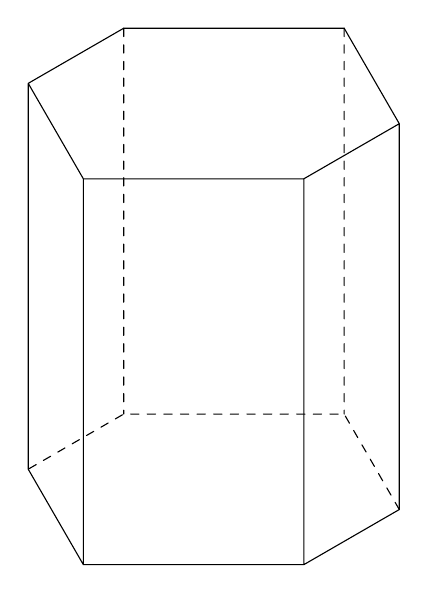
\begin{tikzpicture}[scale=.7, font=\footnotesize, line join=round, line cap=round, >=stealth]
			\def\a{4} \def\b{3}
			\path 
			(0:0) coordinate (A)
			(0:\a) coordinate (B)
			++ (30:\a/2) coordinate (C)
			++ (120:\a/2) coordinate (D)
			++ (180:\a) coordinate (E)
			++ (210:\a/2) coordinate (F)
			\foreach \x in {A,B,C,D,E,F}{(\x)++(-90:7) coordinate (\x_1)}
			;
			\draw (A)--(B)--(C)--(D)--(E)--(F)--cycle
			(A)--(A_1) (B)--(B_1) (C)--(C_1) (F)--(F_1)--(A_1)--(B_1)--(C_1)
			;
			
			\draw[dashed] (D)--(D_1) (E)--(E_1) (C_1)--(D_1)--(E_1)--(F_1);
			%\draw (15:\a) arc(0:360:{\a/2} and {\b/5});
		\end{tikzpicture}
		}
	}
\end{bt}
